\documentclass[a4paper,11pt]{book}
\usepackage{import}
\usepackage{preamb}

\makeindex

\begin{document}

\small
\begin{multicols}{3}

%\maketitle

\thispagestyle{empty}
\scriptsize
\newpage


\begin{subbox}{subbox}{}
\centering
\Large{\textbf{Network Science   \\ Cheatsheet}}
\end{subbox}

\begin{multibox}{2}
\begin{subbox}{subbox}{}
\centering

\includegraphics[width=0.8\textwidth]{pics/logo.png}
\end{subbox}
\begin{subbox}{subbox}{}
\centering
Made by \\
\large{
Remy Cazabet
}
\end{subbox}
\end{multibox}
% \section{Blocks and Community structure}


\begin{subbox}{subbox}{}
\centering
\Large{\textbf{Graph Convolutional Networks}}
\end{subbox}

\begin{subbox}{subbox}{Disclaimer}
Graph Convolutional Networks and Graph Neural Networks in general are a recent field of research, with hundreds of publications in the last few years, and scores of new papers published in every machine learning and network science conference. This class is thus only an introduction to the mechanism underlying the most simple of these approaches.
\end{subbox}


\begin{textbox}{Graph Convolutional Networks}
Graph Convolutional Networks\footcite{zhang2019graph} (GCN) are Deep Neural Networks (NN) designed to work with graphs. They are based on the principle of \textit{propagation} on networks and are especially useful for machine learning tasks such as node classification, although they can be adapted for other tasks. GCN are a subset of a more general field of research called Graph Neural Networks (GNN)\footcite{wu2020comprehensive}
\end{textbox}

\begin{textbox}{Artificial Neural Networks}
Artificial Neural Networks are a family of machine learning algorithms loosely inspired by biological neural network. They are composed of basic units called \textbf{neurons} or \textbf{perceptrons}, that individually play a role equivalent to a logistic classifier: they can be trained through examples to combine \textit{input features} in order to predict a value or a class. A neural network consists in stacking such perceptrons in layers: the \textbf{output} of a perceptron is the \textbf{input} of another one. Layers are separated by non-linear functions called \textbf{activation functions}. All weights are trained simultaneously, allowing to learn \textbf{non-linear}, complex functions.
\end{textbox}

\begin{textbox}{Neural Network Training}
Training a neural network is the same principle as training a linear/logistic regression: the goal is to find weights that minimize a loss function, i.e., a distance, for all pairs input features/target value in a training set, between the target value and the output of the NN when provided the feature values.
\end{textbox}


\begin{textbox}{Deep Neural Networks}
Deep Neural Networks is a name for neural networks composed of a large number of layers of neurons: for instance, a 4-10-2 neural network is composed of 3 layers, the first one composed of 4 neurons (receiving as input data features), whose outputs are the input of 10 neurons in the second layer, whose output are the inputs of 2 neurons in the third and last layer.
\end{textbox}




\begin{textbox}{Fully Connected Layer}
Several types of layers exist. The simplest one is called a Fully connected layers, and is simply defined such as all the outputs of each neuron in a layer are inputs of the neurons of the next layer.
\end{textbox}


\begin{textbox}{Illustration of a Neural Network}

\centering

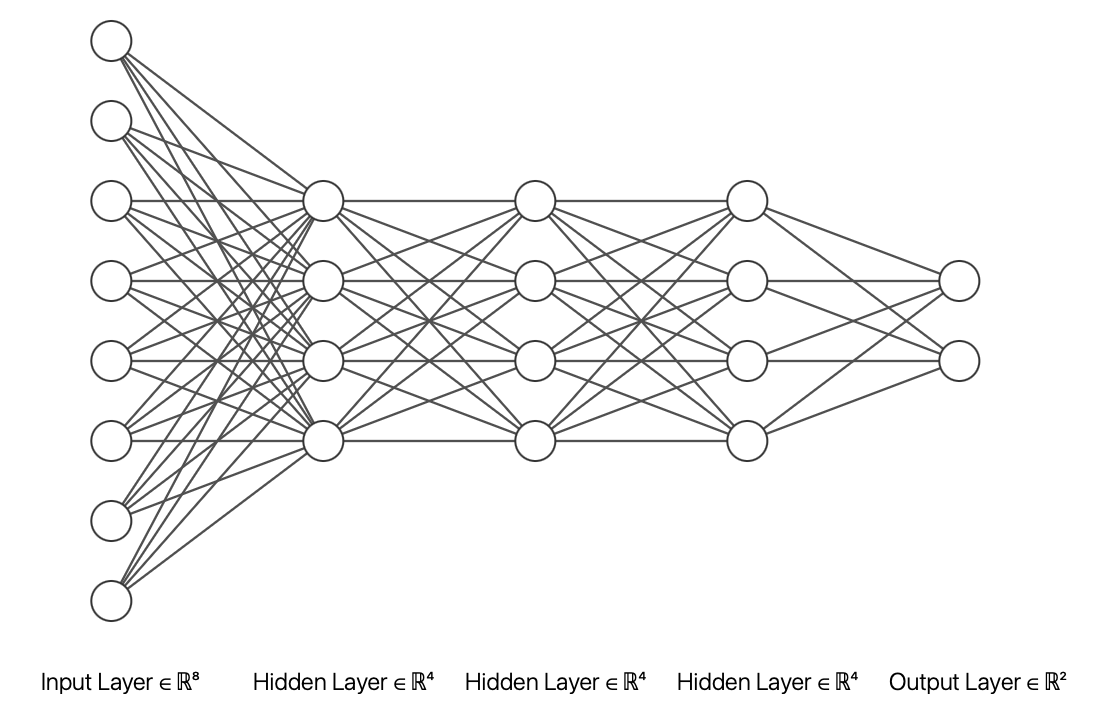
\includegraphics[width=0.7\linewidth]{pics/NN_SVG.png}

A deep neural networks composed of 3 hidden layers. The input is provided as 8 features, each of the hidden layer has 4 neurons, and they are fully connected layers. The output consists of 2 output values.
\end{textbox}


\begin{textbox}{Convolution Layer}
\textbf{Convolution layers} are another type of layers in which inputs are combined in a particular way, based on some relation known \textit{a priori} between them. They are typically used on images: each pixel of the image is a feature (e.g.: from 0 --white-- to 255 --black), and those pixels have a particular organization: each pixel has 4 (rook adjacency]) or 8 (Queen adjacency) neighbors. 

In a convolution layer, a \textbf{higher level} pixel is created for each input pixel by combining its neighbors in a particular way. The matrix defining how to combine neighbors is called a \textbf{kernel}.
\end{textbox}

\begin{textbox}{Illustration of a convolution}
\centering
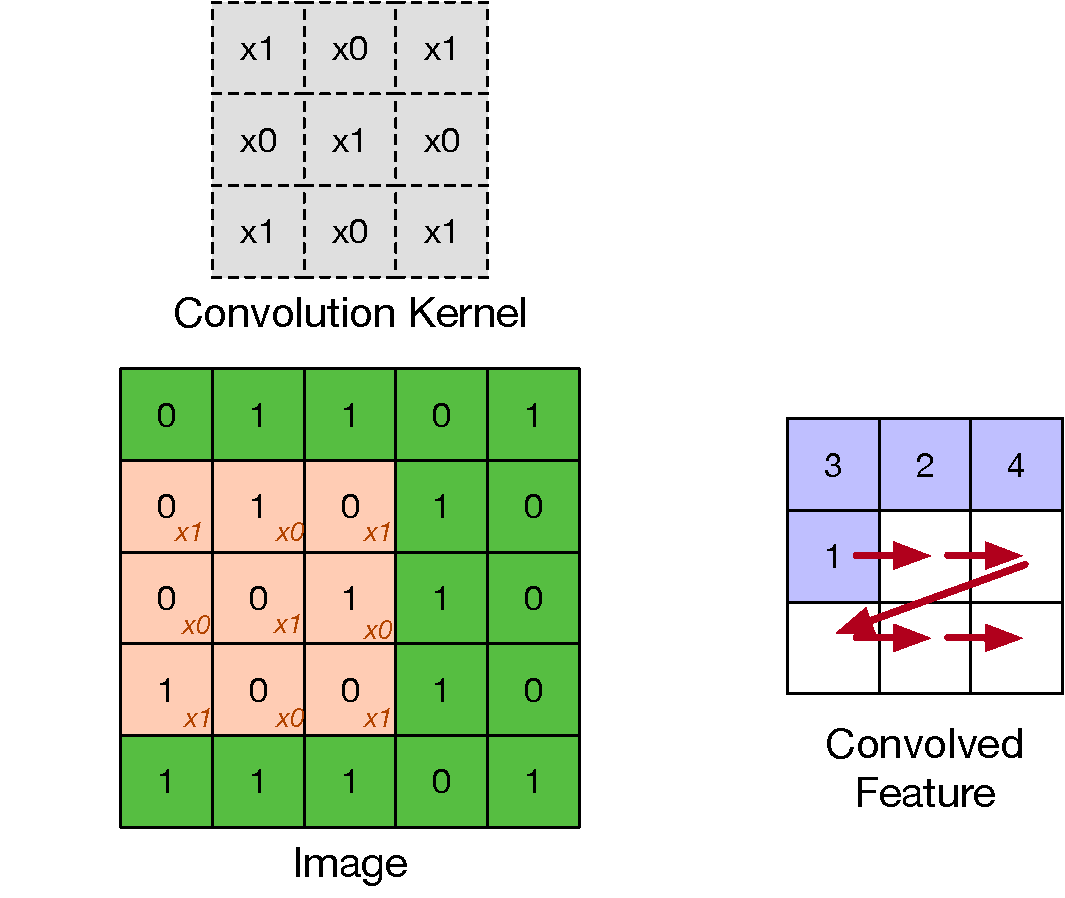
\includegraphics[width=0.6\linewidth]{pics/convolution.pdf}
\end{textbox}

\begin{textbox}{Example of kernels}
\centering
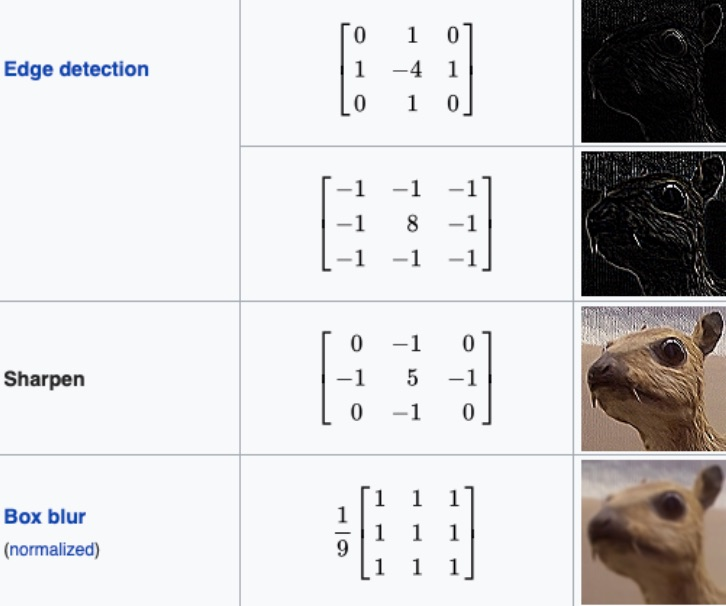
\includegraphics[width=0.8\linewidth]{pics/kernels.jpg}
\footnote{\url{https://en.wikipedia.org/wiki/Kernel_(image_processing)}}
\end{textbox}

\begin{textbox}{Trainable kernels}
In neural networks, the kernel used in a layer is not chosen \textit{a priori}, its weights are learned to minimize the global prediction error, as any other weight.
\end{textbox}

\begin{textbox}{Convolution - intuition}
The intuition of stacking several convolution layers is to learn higher levels of abstraction at every layer. Intuitively, the first layer might recognize lines and curves, the second circles and simple patterns, the third, eyes, letters or composed shapes, until the last one can recognize animals or faces, for instance.
\end{textbox}

\begin{textbox}{Images as graphs}
Intuitively, the relation between pixels in an image can be represented by a graph: each pixel is represented by a node, and each node is connected to neighboring pixels in the picture. The corresponding graph is thus a regular grid.

\centering
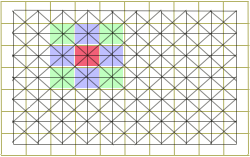
\includegraphics[width=0.5\linewidth]{pics/picture_graph.png}

Pixels of an image in yellow, graph corresponding to pixel direct proximity (diagonals and lateral) in black.
\end{textbox}



\begin{textbox}{Graph Convolution}
The concept of convolution can be extended to any graph. A \textbf{Graph convolutional layer} computes a value for each node by combining the values of its neighbors. Note that each node can have a different number of neighbors, thus instead of combining directly the values of the neighbors, the kernel combines the average values of the neighbors. e.g, if each node has 10 features, we first compute the average value among neighbors for each feature, and then the kernel controls how to combine those average values.
%\centering
%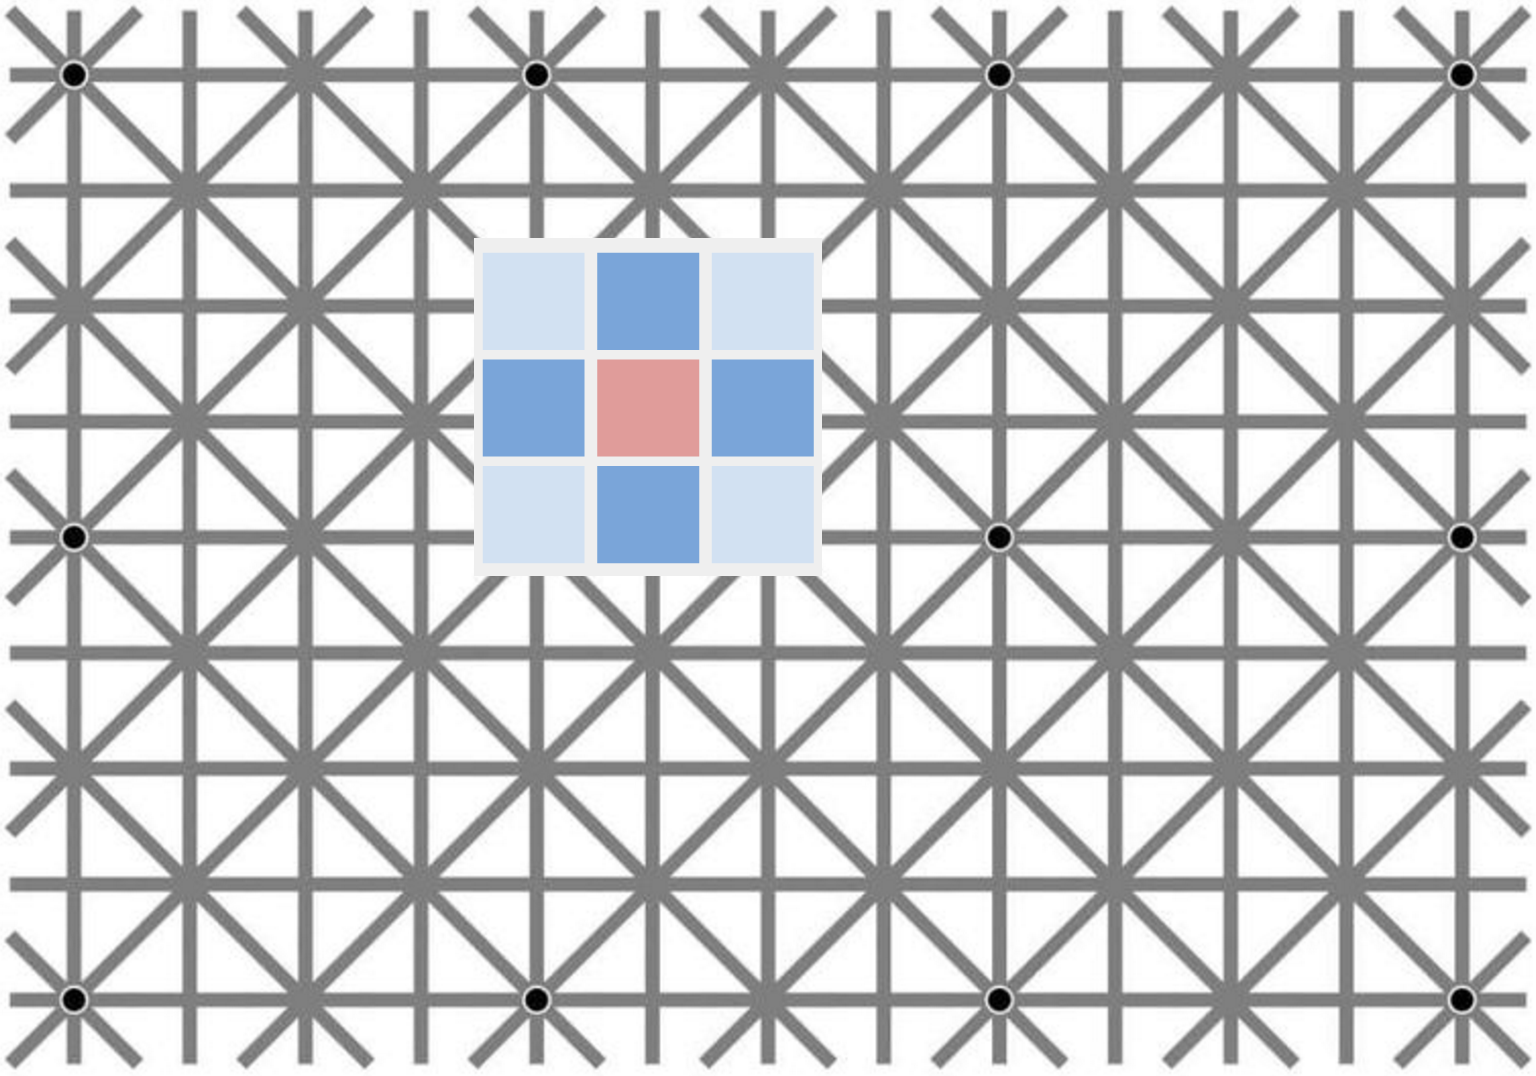
\includegraphics[width=0.5\linewidth]{pics/graphgrid.png}

%Image Convolution VS Graph Convolution

\end{textbox}



\begin{textbox}{Convolution and diffusion}
There is a strong relation between a graph convolutional layer and diffusion in networks. Training a graph convolutional layer consists in learning the best way for nodes to combine the features of their neighbors to make predictions, according to the training examples.
\end{textbox}


\begin{textbox}{Stacking GCN layers}
A single GCN layer combines, for each node, values of its direct neighbors. With 2 layers, the value of a node is computed from nodes at distances up to 2 in the graph. The more successive layers, the farther in the graph a node can influence other nodes. Remember that in most real graphs, the average shortest path is small, thus 5 or 6 layers can be enough for most nodes to influence most other nodes.
\end{textbox}



\begin{textbox}{Graph Convolutional Layer: Definition}
The typical Graph Convolutional Layer \footcite{kipf2016semi} is defined as follows:
\[
f(H^{(l)}, A) = \sigma\left( \hat{D}^{-\frac{1}{2}}\hat{A}\hat{D}^{-\frac{1}{2}}H^{(l)}W^{(l)}\right)
\]

We will decompose this equation do understand what it does.

\end{textbox}

\begin{textbox}{Feature Matrix $H$}
Graph Convolution uses node \textit{features} to make predictions on nodes. Nodes features are represented by a Matrix $H$. $H_i$ corresponds to the vector of features of node $i$. Features can be attributes (age, political opinion, etc.) or structural properties (centralities, etc.). Matrix $H$ is of shape $n\times d$, with $n$ the number of nodes and $d$ the number of features.
\end{textbox}


\begin{textbox}{Feature Combination $AH$}
The GCN layer consists for each node in combining its neighbors features. $AH$ is the simplest way of doing this combination, it computes for each node a vector, corresponding to the sum of the vectors of its neighbors. For instance, if each node originally has 2 features, age and degree, after the $AH$ operation, the vector $H'_i$ of node $i$ is composed of 2 values, the sum of age of its neighbors, and the sum of degrees of its neighbors. The matrix $H'$ is thus of shape $n\times d$. 

To avoid nodes with high degrees having systematically higher values, we usually use instead a \textbf{normalized adjacency matrix} to compute \textbf{average values}.
\end{textbox}


\begin{textbox}{Adding self loops $\hat{A}$}
Until now, we have said that a GCN combines the features of its neighbors. However, in most cases, the features of the node itself are also relevant. Let's assume that we want to predict an individual $i$ \textit{revenue} from available \textit{age} and \textit{betweenness} information. Using the neighbors age and betweenness is meaningful, but using age and betweenness of $i$ itself is probably relevant too. We represent this by saying that each node is also a neighbor of itself, i.e., in graph terms, we add a self-loop to each node. In matrix term, we replace $A$ by $\hat{A}=A+I$ with $I$ the identity matrix (values on the diagonal are all 1, and all other values are 0).
\end{textbox}



\begin{textbox}{Normalized Adjacency Matrix $\hat{D}^{-\frac{1}{2}}\hat{A}\hat{D}^{-\frac{1}{2}}$}

In order to compute the \textbf{average} of neighbors features instead of the sum, we can use a normalized adjacency matrix, by multiplying it by the inverse of the Degree matrix $D^{-1}$, i.e., a matrix such as $D_{ii}=\frac{1}{k_i}$, and all other values are 0. 

$D^{-1}\hat{A}H$ computes the average of neighbors features. However, in many cases, it is more meaningful to use an average weighted by the degree, i.e., neighbors with small degrees have more influence than neighbors of large degrees. As for heuristics like Adamic Adar, it can be interpreted by doing a parallel with social networks: To infer a node revenue from age of neighbors, the age of my close friends (low degrees) is probably more meaningful than the age of the pop-stars (high degrees) I follow. This weighted average is computed by the normalized Adjacency matrix: 

\[
D^{-\frac{1}{2}}\hat{A}D^{-\frac{1}{2}}
\]

\end{textbox}




\begin{textbox}{ $\hat{D}^{-\frac{1}{2}}\hat{A}\hat{D}^{-\frac{1}{2}}$ - visually}
\begin{multibox}{2}

\begin{subbox}{subbox}{}
\centering
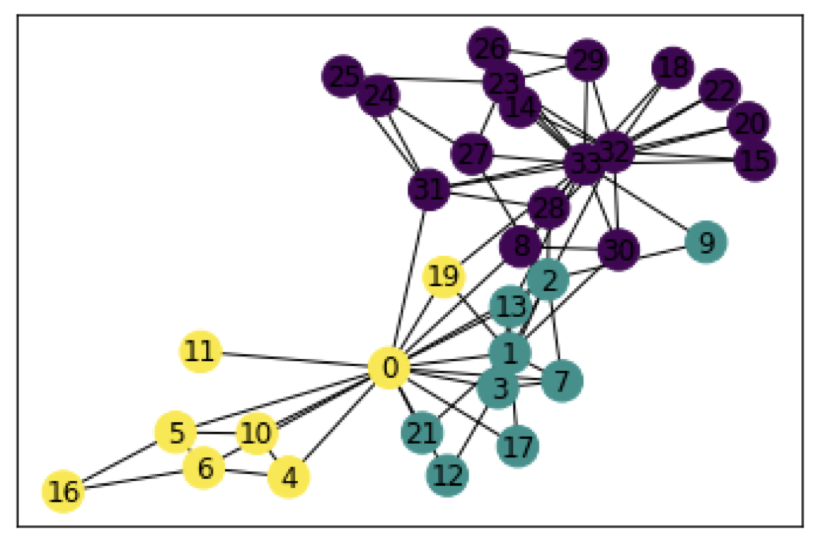
\includegraphics[width=1\linewidth]{pics/Akarate.png}

$G$
\end{subbox}
\begin{subbox}{subbox}{}
\centering
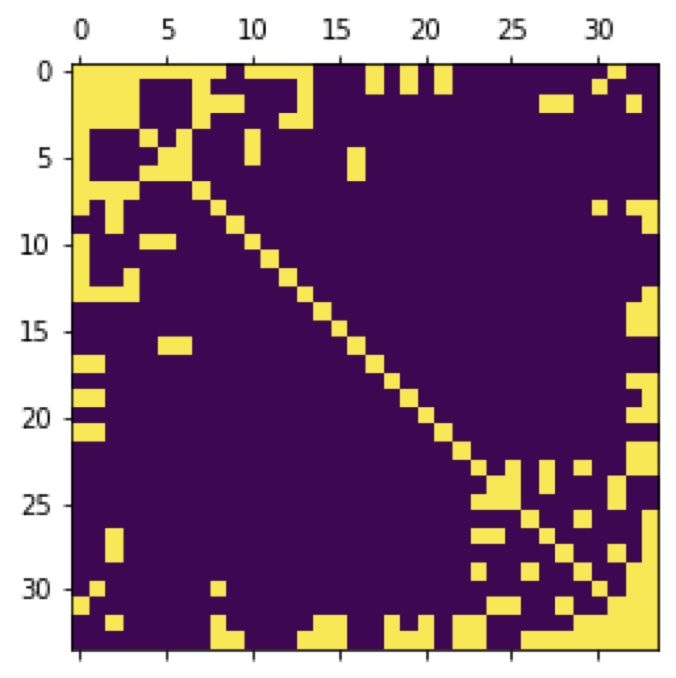
\includegraphics[width=0.95\linewidth]{pics/A.png}

$\hat{A}$
\end{subbox}
\end{multibox}

\begin{multibox}{2}

\begin{subbox}{subbox}{}
\centering
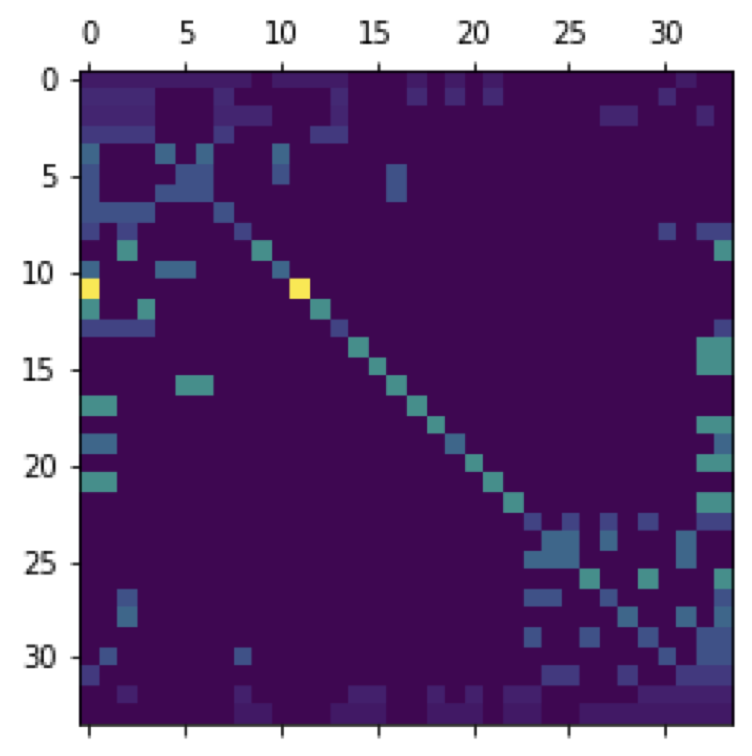
\includegraphics[width=1\linewidth]{pics/DA.png}

$D^{-1}\hat{A}$
\end{subbox}
\begin{subbox}{subbox}{}
\centering
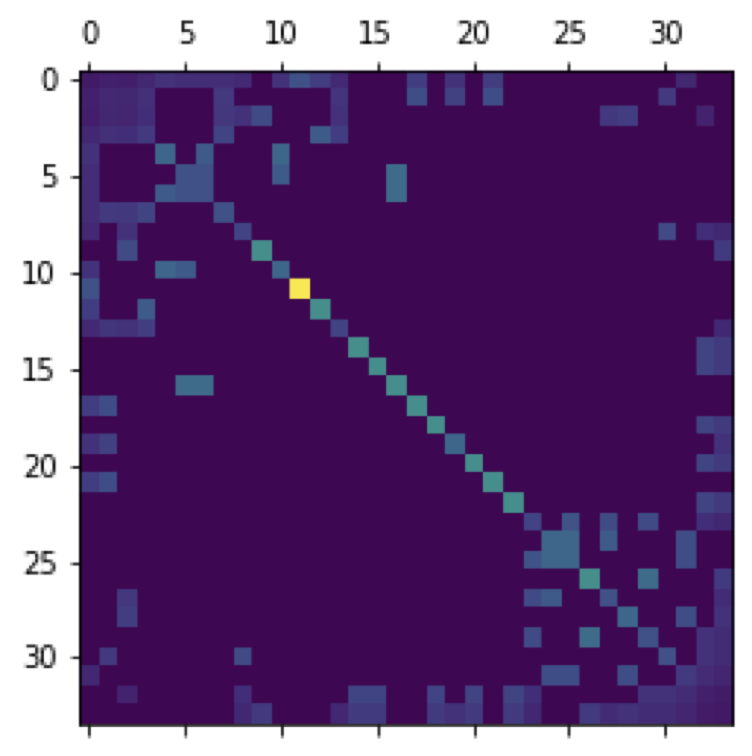
\includegraphics[width=1\linewidth]{pics/DAD.png}

$D^{-\frac{1}{2}}\hat{A}D^{-\frac{1}{2}}$
\end{subbox}

\end{multibox}

\end{textbox}








\begin{textbox}{Weight Matrix $W$ - Single layer}
Let's note $H'$ the result of the averaging of the neighbors features. $H'_i$ is the vector of averaged values of node $i$. $H'W$ computes new features for each node by combining its neighbors features. For instance, consider that we have $d=3$ features, e.g., age, betweenness and degree. If we have a single GCN layer and we want to predict a single variable, e.g., the revenue, then $W$ could be of shape $d\times 1$, and each node $i$ predicted value is $H'_{1i}w_1+H'_{2i}w_2+H'_{3i}w_3$, with $H'_{1i},H'_{2i},H'_{3i}$ respectively the average age, betweenness and degree of the neighbors of $i$, and $w_1,w_2,w_3$ learned weights, shared for every node.
\end{textbox}



\begin{textbox}{Weight Matrix $W$ sizes - Multiple layers}
In most cases, GCN layers are chained one after the other. At each level, a different weight matrix is used, that we can note $W_l$ for level $l$.

The size of those matrices is determined as follows: The first dimension is the number of features in \textbf{input} of the layer. The second dimension is the number of features wanted in \textbf{output} of the layer. For instance, if we originally have 10 features for each node, we can design a 3 layer neural network with weight matrix sizes: $W_1$:$10\times 10$, $W_2$:$10\times 5$, $W_3$:$5\times 1$. 

This network first transforms the 10 original features in 10 new features that are combinations of the neighbors features, then these 10 features are combined into 5, and finally those 5 features are combined into a single one.
\end{textbox}




\begin{textbox}{Activation function $\sigma$}
The last element of the GCN layer is the activation function $\sigma$. Activation function are commonly used between layers in deep neural networks, to add non-linearity. With GCN, the most commonly used is the \textbf{ReLu} (\textit{Rectified Linear Unit}), which is defined as:
 \[
    \sigma(x) = \begin{cases}
        x, & x > 0\\
        0, & x\leq 0\\
        \end{cases}
  \]
 Intuitively, it mimics the behavior of biological neurons: if the value is above a threshold, the network \textit{fires}, and its value is propagated to the the next layer, if not, the computed value is lost.

\end{textbox}

\begin{textbox}{No feature}
If no feature is available for nodes, it has been proposed to use $H=I$. Since by definition $AI=A$, the average of neighbor's features of node $i$ is $A_i$.
\end{textbox}


\begin{textbox}{Weight initialization}
The objective of the machine learning process is to learn the weight matrix $W$. $W$ is typically initialized with random values, generated by a Normal distribution centered on 0. Negative values are required to benefit from the ReLU activation function.
\end{textbox}



\begin{textbox}{Forward and Backward steps}
We call \textbf{Forward step} the computation of layers in sequence, for fixed values of $W_l$. 

We call Backward step the update of $W_l$ matrices. These updates are done using a technique called \textbf{back-propagation}, whose objective is to minimize the loss function (error) between the result of the forward step and the objective result (known from a training set)
\end{textbox}

\begin{textbox}{Example of a forward step}
Let's look at the forward step of a simple network. The graph structure is the Zackary Karate Club. We consider no features, and thus use $H=I$. We set 2 GCN layers: $l_1$ converts from $n$ dimensions to 5 dimensions, $l_2$ converts from 5 dimensions to 2 dimensions.

\centering
\textbf{First Layer}
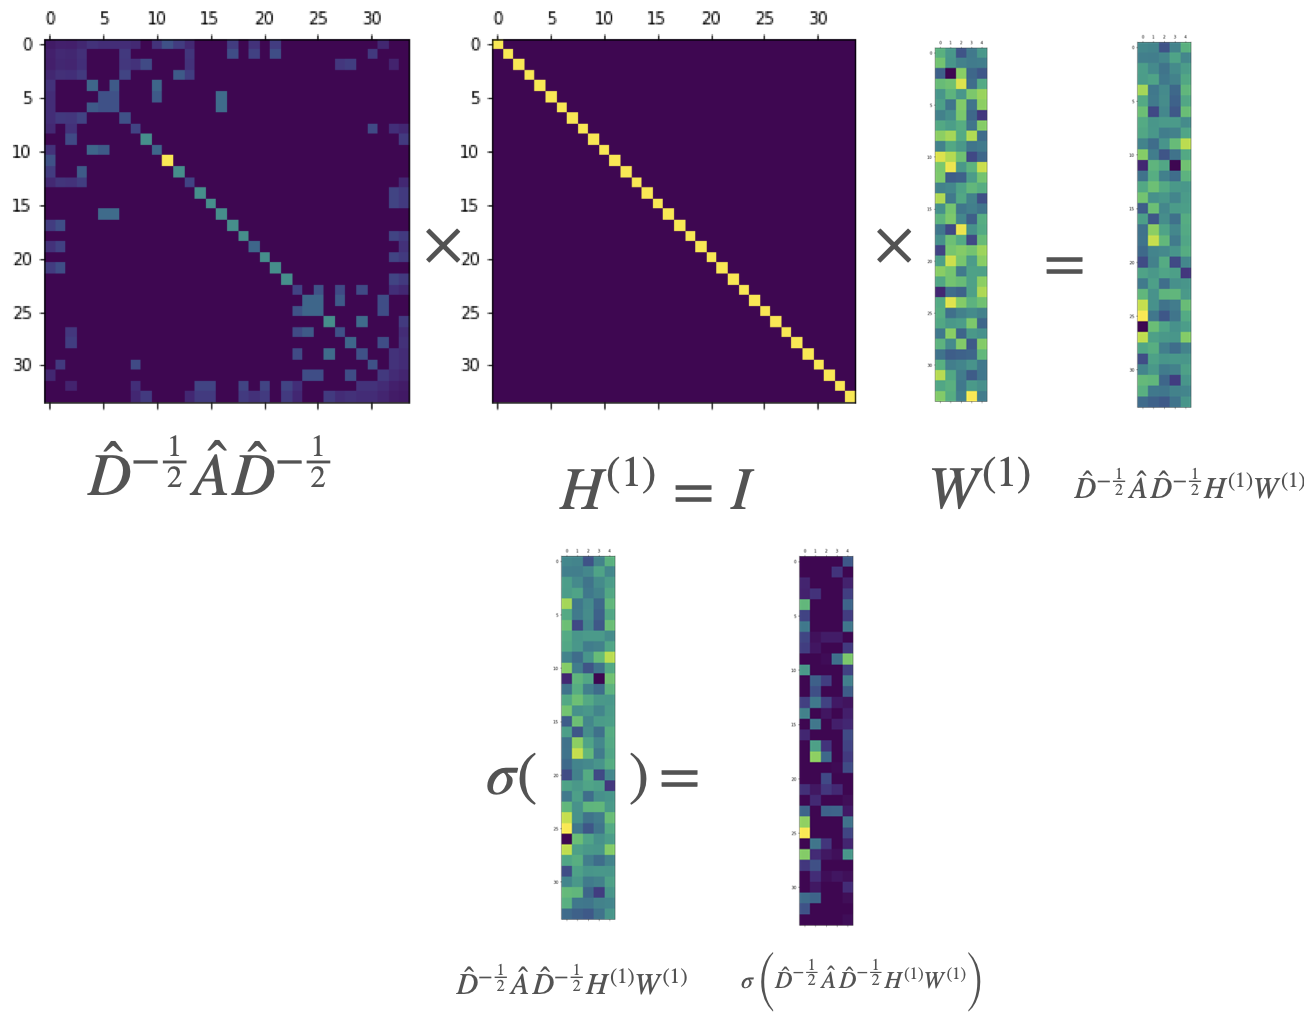
\includegraphics[width=1\linewidth]{pics/forward1.png}
\centering

\textbf{Second Layer}

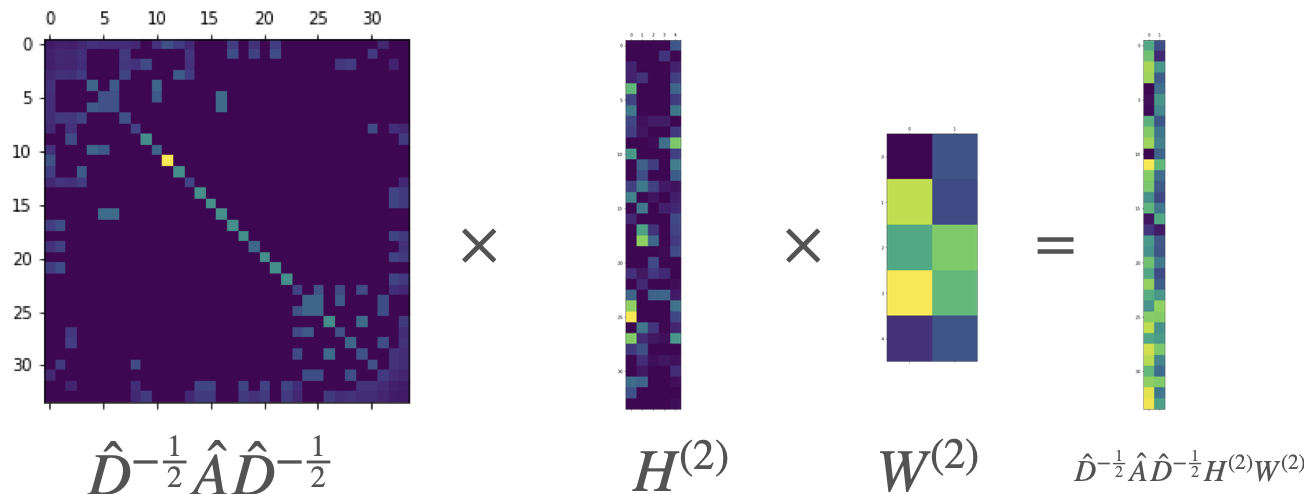
\includegraphics[width=1\linewidth]{pics/forward2.png}
\end{textbox}


\begin{textbox}{Forward step embedding}
After the forward propagation, \textbf{without} weight learning, we obtain in our example a result that can be interpreted as a 2 dimensional embedding. 

\centering
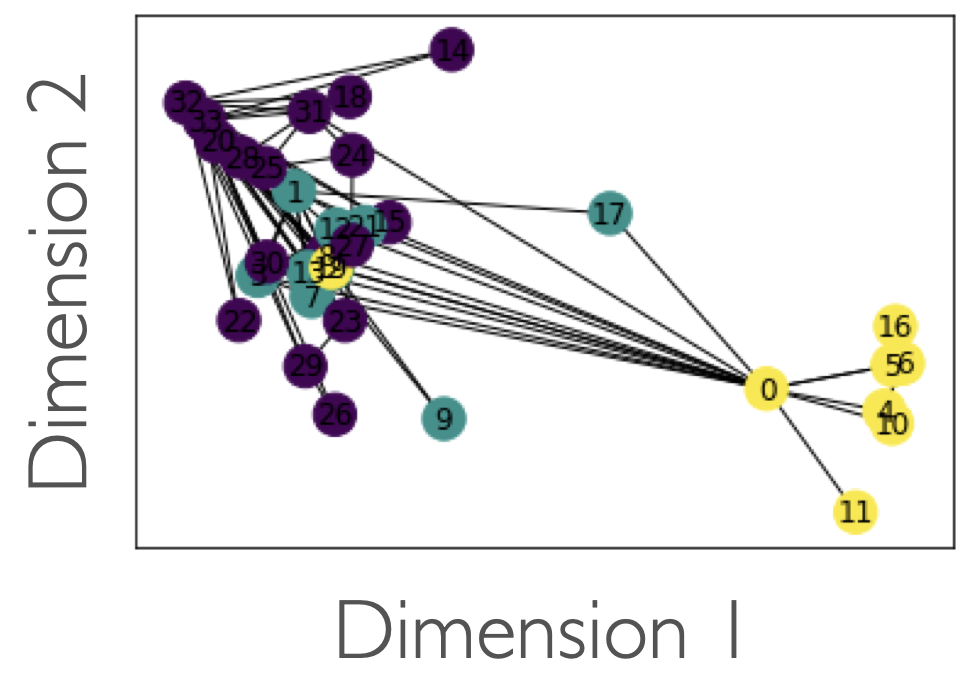
\includegraphics[width=0.7\linewidth]{pics/karateEmbedd.png}

We can note, despite random weights, that the forward process seems to capture some network structure.
\end{textbox}


\begin{textbox}{Weight learning - Backpropagation}
To learn the weight matrices, one requires: 
\begin{itemize}
    \item Examples of desired outputs for some nodes (ground truth label)
    \item A \textbf{loss function}, i.e., a function to measure the difference between the true labels and the labels produced by the forward step
\end{itemize}
At each step, a \textbf{gradient descent} approach is used: knowing the \textbf{derivative} of the loss function, weights are updated in the direction that reduces the loss, such as a new forward step with those updated weights would produce a result closer to the true labels. 
\end{textbox}



\begin{textbox}{Example: ZKC node clustering}
The \textbf{Zackary Karate Club} (\textbf{ZKC}) is a famous network dataset. It represents social relations in a Club of Karate, that were collected before the two instructors decide to split apart, each creating his own club, attracting approximately half  the students of the original club. It is often used as a toy application case for community detection/Network clustering, were the task is to identify the students that will follow each teacher, from the social graph observed before the split.
\end{textbox}


\begin{textbox}{ZKC as a semi-supervised Problem}
To formalize the ZKC task as a classification problem, we label each of the two instructors (nodes 0 and 33) with opposed labels (0 and 1). Starting with the same setting as earlier, i.e., $I$ matrix as features, we optimize the weights of the 2 GCN layers in order to minimize the difference between the labels of the teachers and the output of the Graph Neural Network. Note that we kept a vector of size 2 in output, with opposite objectives (for the first, instructors labels are (0,1), for the second, (1,0).)
\end{textbox}


\begin{textbox}{Trained weights}
\centering

Trained weights of first and second layers, and output vectors (2 dimensions).
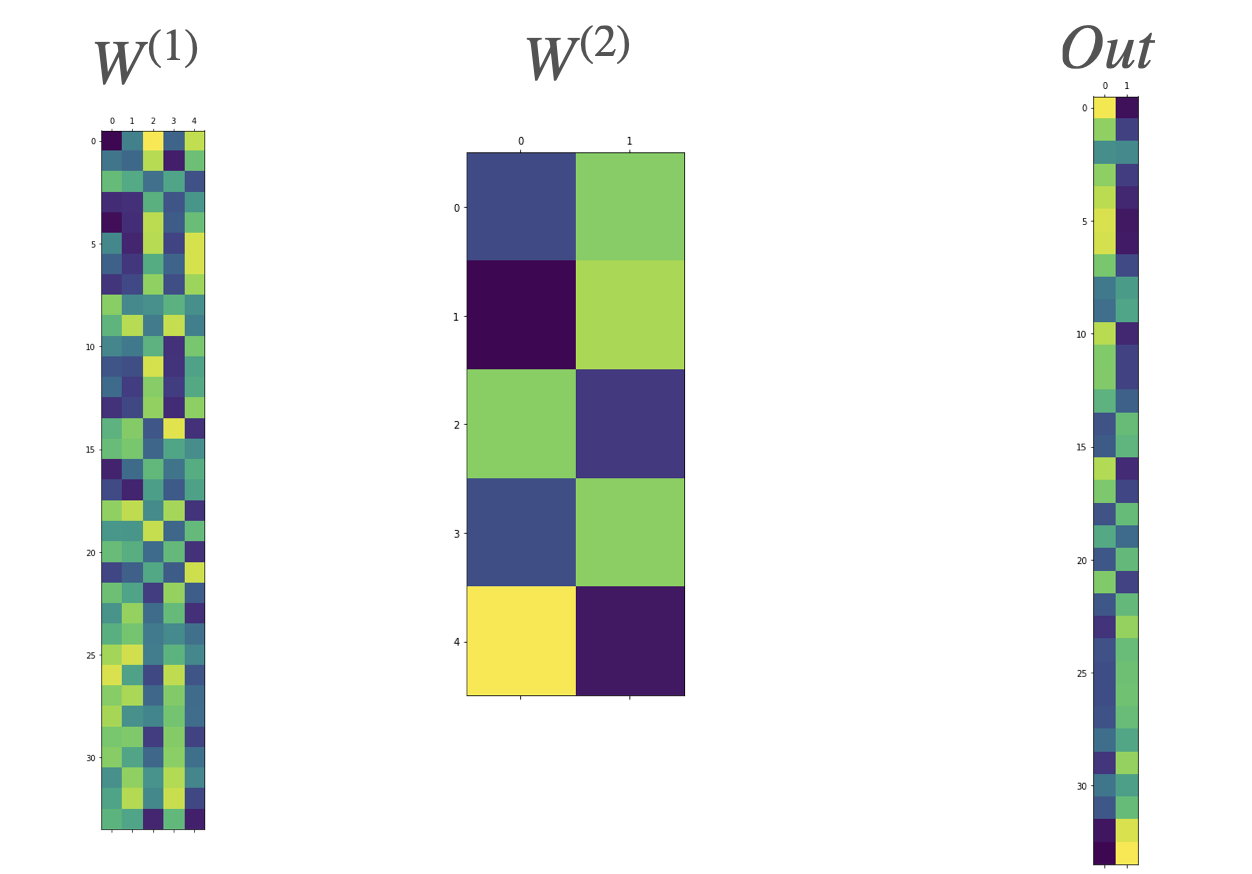
\includegraphics[width=0.8\linewidth]{pics/weights.png}

Note that for the first and last nodes (instructors), vectors in output correspond to the objective (respectively,(1,0) and (0,1)).
\end{textbox}




\begin{textbox}{Clustering}
\centering

Illustration of usages of the vectors obtained after training of the GCN. 

\centering
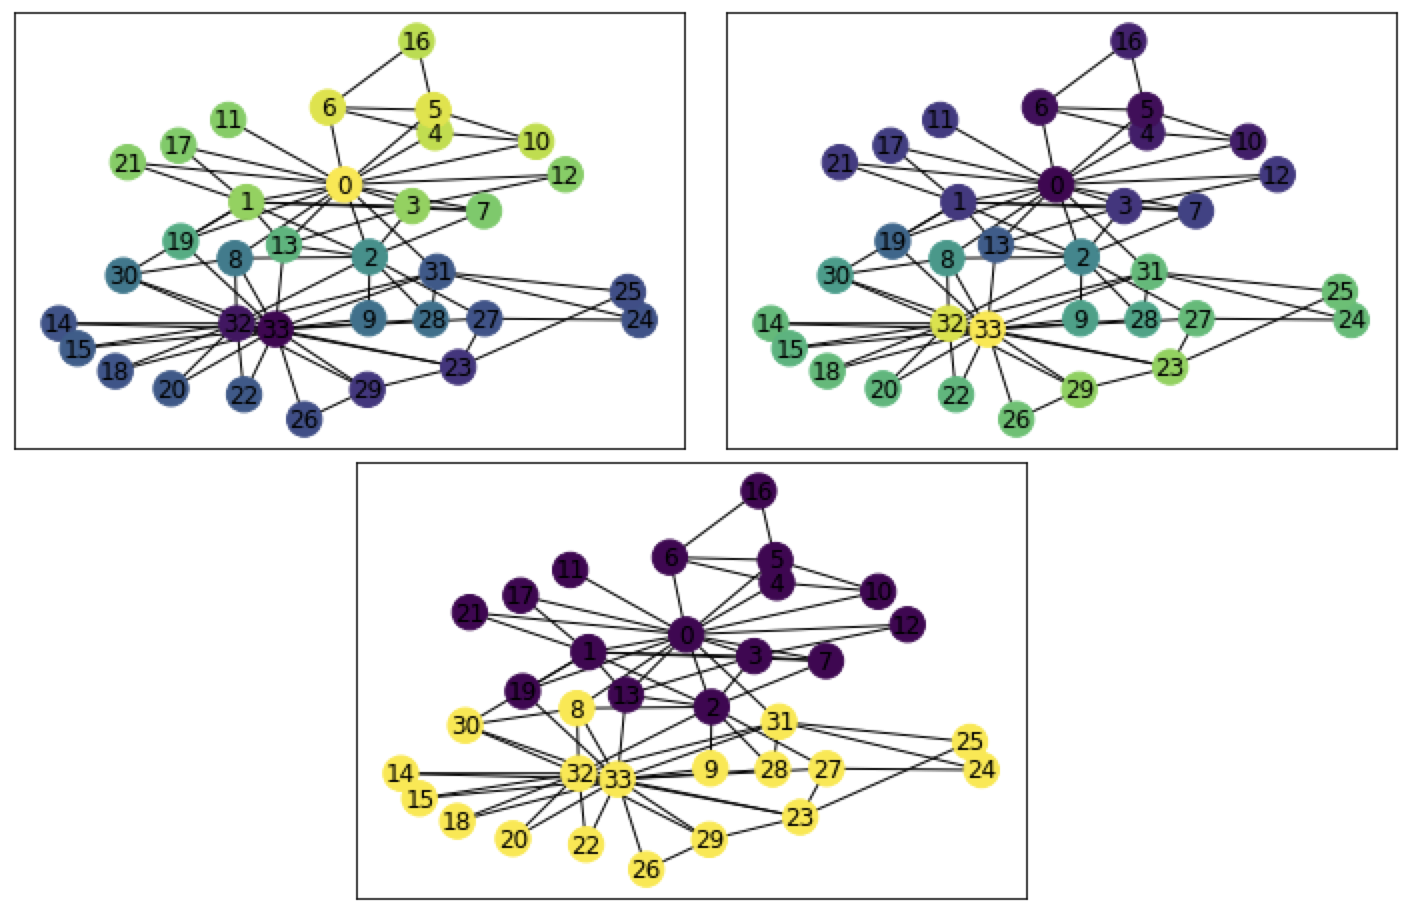
\includegraphics[width=0.8\linewidth]{pics/ZKCGCNresult.png}




\textbf{Top Left}: Values of the first computed feature. \textbf{Top Right}: Values of the second computed feature. \textbf{Bottom}: clustering obtained by assigning each node to the feature for which it has the highest value (example of heuristic).
\end{textbox}





\begin{textbox}{Going Further}
Python library: DGL (\url{https://www.dgl.ai})

Survey GCN: (\cite{zhang2019graph})(\cite{zhang2018graph})

Survey Graph Neural Networks (GNN): (\cite{zhou2018graph})(\cite{wu2020comprehensive})

General presentation of GNN: (\cite{xu2018powerful})

Variational graph Auto-Encoders (\cite{kipf2016variational})

Link Prediction with GNN (\cite{zhang2018link})

DCRNN: Convolutionnal Recurrent GNN (\cite{li2017diffusion})


\end{textbox}


 \AtNextBibliography{\footnotesize}


\printbibliography[heading=subbibliography]


\end{multicols}







\end{document}


